\documentclass{sigchi}

% Use this section to set the ACM copyright statement (e.g. for
% preprints).  Consult the conference website for the camera-ready
% copyright statement.

% Copyright
\CopyrightYear{2020}
%\setcopyright{acmcopyright}
\setcopyright{acmlicensed}
%\setcopyright{rightsretained}
%\setcopyright{usgov}
%\setcopyright{usgovmixed}
%\setcopyright{cagov}
%\setcopyright{cagovmixed}
% DOI
\doi{https://doi.org/10.1145/3313831.XXXXXXX}
% ISBN
\isbn{978-1-4503-6708-0/20/04}
%Conference
\conferenceinfo{CHI'20,}{April  25--30, 2020, Honolulu, HI, USA}
%Price
\acmPrice{\$15.00}

% Use this command to override the default ACM copyright statement
% (e.g. for preprints).  Consult the conference website for the
% camera-ready copyright statement.

%% HOW TO OVERRIDE THE DEFAULT COPYRIGHT STRIP --
%% Please note you need to make sure the copy for your specific
%% license is used here!
% \toappear{
% Permission to make digital or hard copies of all or part of this work
% for personal or classroom use is granted without fee provided that
% copies are not made or distributed for profit or commercial advantage
% and that copies bear this notice and the full citation on the first
% page. Copyrights for components of this work owned by others than ACM
% must be honored. Abstracting with credit is permitted. To copy
% otherwise, or republish, to post on servers or to redistribute to
% lists, requires prior specific permission and/or a fee. Request
% permissions from \href{mailto:Permissions@acm.org}{Permissions@acm.org}. \\
% \emph{CHI '16},  May 07--12, 2016, San Jose, CA, USA \\
% ACM xxx-x-xxxx-xxxx-x/xx/xx\ldots \$15.00 \\
% DOI: \url{http://dx.doi.org/xx.xxxx/xxxxxxx.xxxxxxx}
% }

% Arabic page numbers for submission.  Remove this line to eliminate
% page numbers for the camera ready copy
% \pagenumbering{arabic}

% Load basic packages
\usepackage{balance}       % to better equalize the last page
\usepackage{graphics}      % for EPS, load graphicx instead 
\usepackage[T1]{fontenc}   % for umlauts and other diaeresis
\usepackage{txfonts}
\usepackage{mathptmx}
\usepackage[pdflang={en-US},pdftex]{hyperref}
\usepackage{color}
\usepackage{booktabs}
\usepackage{textcomp}
\usepackage{graphicx}
\usepackage[table]{xcolor}
\usepackage{tabularx}

% Some optional stuff you might like/need.
\usepackage{microtype}        % Improved Tracking and Kerning
% \usepackage[all]{hypcap}    % Fixes bug in hyperref caption linking
\usepackage{ccicons}          % Cite your images correctly!
% \usepackage[utf8]{inputenc} % for a UTF8 editor only

% If you want to use todo notes, marginpars etc. during creation of
% your draft document, you have to enable the "chi_draft" option for
% the document class. To do this, change the very first line to:
% "\documentclass[chi_draft]{sigchi}". You can then place todo notes
% by using the "\todo{...}"  command. Make sure to disable the draft
% option again before submitting your final document.
\usepackage{todonotes}

% Paper metadata (use plain text, for PDF inclusion and later
% re-using, if desired).  Use \emtpyauthor when submitting for review
% so you remain anonymous.
\def\plaintitle{Promoting Health Using VR/AR}
\def\plainauthor{Aaron Marquez, Adan Soto, Antony Smelianski, Trevon Donsereaux}
\def\emptyauthor{}
\def\plainkeywords{Virtual reality; physical activity; heart rate; oculus quest}
\def\plaingeneralterms{Documentation, Standardization}

% llt: Define a global style for URLs, rather that the default one
\makeatletter
\def\url@leostyle{%
  \@ifundefined{selectfont}{
    \def\UrlFont{\sf}
  }{
    \def\UrlFont{\small\bf\ttfamily}
  }}
\makeatother
\urlstyle{leo}

% To make various LaTeX processors do the right thing with page size.
\def\pprw{8.5in}
\def\pprh{11in}
\special{papersize=\pprw,\pprh}
\setlength{\paperwidth}{\pprw}
\setlength{\paperheight}{\pprh}
\setlength{\pdfpagewidth}{\pprw}
\setlength{\pdfpageheight}{\pprh}

% Make sure hyperref comes last of your loaded packages, to give it a
% fighting chance of not being over-written, since its job is to
% redefine many LaTeX commands.
\definecolor{linkColor}{RGB}{6,125,233}
\hypersetup{%
  pdftitle={\plaintitle},
% Use \plainauthor for final version.
%  pdfauthor={\plainauthor},
  pdfauthor={\emptyauthor},
  pdfkeywords={\plainkeywords},
  pdfdisplaydoctitle=true, % For Accessibility
  bookmarksnumbered,
  pdfstartview={FitH},
  colorlinks,
  citecolor=black,
  filecolor=black,
  linkcolor=black,
  urlcolor=linkColor,
  breaklinks=true,
  hypertexnames=false
}

% create a shortcut to typeset table headings
% \newcommand\tabhead[1]{\small\textbf{#1}}

% End of preamble. Here it comes the document.
\begin{document}

\title{\plaintitle}

\numberofauthors{4}
\author{
  \alignauthor{Aaron Marquez\\
    \affaddr{Colorado State University}\\
    \affaddr{Fort Collins, Colorado}\\
    \email{azmarque@rams.colostate.edu}}\\
  \alignauthor{Adan Soto\\
    \affaddr{Colorado State University}\\
    \affaddr{Fort Collins, Colorado}\\
    \email{asoto98@rams.colostate.edu}}\\
  \alignauthor{Antony Smelianski\\
    \affaddr{Colorado State University}\\
    \affaddr{Fort Collins, Colorado}\\
    \email{asmelian@rams.colostate.edu}}\\
  \alignauthor{Trevon Donsereaux\\
    \affaddr{Colorado State University}\\
    \affaddr{Fort Collins, Colorado}\\
    \email{tdons@rams.colostate.edu}}\\
}

\maketitle
\begin{abstract}
    Created a virtual reality game that emulates dodgeball. This was done in efforts of promoting physical health in a world where obesity is at an all time high. Using unity the game was created and programmed to throw dodgeballs to the player spawned on a basketball court. Said dodgeballs spawned at different places and moved towards the player at speeds within a range. Procedure consisted of having users do a trial outdoors playing the real-life game followed by a trial indoors using an Oculus Quest. It was found that our results were inconclusive due to the sample size being too low because of the ongoing pandemic.
\end{abstract}

% ACM Classfication
\begin{CCSXML}
<ccs2012>
<concept>
<concept_id>10003120.10003121.10003124.10010866</concept_id>
<concept_desc>Human-centered computing~Virtual reality</concept_desc>
<concept_significance>500</concept_significance>
</concept>
</ccs2012>
\end{CCSXML}

\ccsdesc[500]{Human-centered computing~Virtual reality}
\ccsdesc[300]{Human-centered computing~User Studies}

% Author Keywords
\keywords{\plainkeywords}

% Print the classficiation codes, codes @ https://dl.acm.org/ccs/ccs_flat.cfm
\printccsdesc

\section{Introduction}
Between 2017-2018, the prevalence of obesity was 42.4\% within the United States alone and continues to grow.\cite{CDC_2020} Given the increase in obesity and the common lack of physical activity among Americans and people of the world, we developed a project that aims to tackle this problem by giving users the opportunity to exercise at any given time while making it seem like a videogame. This is so that the feeling of playing a videogame makes the user forget the fact that they are working out. It is known that this is of current interest in the world of gaming and decided to attempt to solve the problem with our own approach\cite{mcclure_schofield}. In order to facilitate the interest of exercise through gaming our project had to be interesting and engaging enough to get people to actually partake in the game. By using newer technologies like VR, the goal was to bring enough interest/wow factor by users to actually pursue trying the game. With the available technologies and widely known platforms such as Unity and hardware like the Oculus Quest, our project came together but this was not an easy task. 

There were many roadblocks our team had to get through, some were faced as soon as we began work due to the complicated set up of unity and the initial structure we had for the project, but this was only the beginning of more obstacles to come our way. Working during these tough times made this project and overall semester much more difficult due to the added stress of this virus that is still taking lives all over the world. It is also worth mentioning that all of our team members had never been exposed to any kind of virtual reality tools so getting started and making the originally desired progress was unfortunately not possible. 

Even with all of the mentioned setbacks, our team was able to create a great looking game that met our initial goal although not with all of the features we were hoping to add. We created a game that keeps the player engaged and sweating since the level of activity can be rigorous at times. The logic behind the game makes sure that the user is able to succeed at the game but not as easily as they may hope. There exists a perfect level of difficulty and finding said difficulty is key to keep the player motivated, much more information will be provided in later sections of the report where a detailed explanation of the code behind the logic of the game will give insight into the inner workings of our game. What follows is a thorough explanation of our project as a whole as well as an examination of experiment’s results used to determine the level of success of our game. 


\subsection{Literature Review}
\subsubsection{Research on Application of Virtual Reality Technology in Competitive Sports}

The Research on Application of Virtual Reality Technology in Competitive Sports journal article\cite{sanz_franck_lecuyer_anatole_ferran_2015} focuses on the potential of Virtual Reality to improve the ability of professional athletes to train harder and more than usual and take their skills to a higher level. It focuses on the important aspects that must be perfected in order for Virtual Reality to be effective as a proper training method. It emphasizes the importance of having accurate opponents with real techniques and strategies as well as mimicking real environments in order for the training. If these factors are correct there is a great benefit that can come from using Virtual Reality technology as another tool in a coach’s toolbox to further develop athletes’ abilities. Although this research might not be directly related to the research being conducted in this paper, it still brings up some relevant issues that must be addressed further into the developing stage, this being the importance of creating an immersive environment. The main focus of the article was taking training and athletes to a higher level and also having the ability to record many different sorts of physiologic and biologic data while they train. Perhaps biologic and physiologic data are not the main focus of this research paper but escalating skill and introducing participants to a specific sport are definitely of interest. The Research on Application of Virtual Reality Technology in Competitive Sports journal article definitely helps pointing this research paper in the right direction by proving many of the factors that make VR appropriate for athletes that can also translate to beginner participants. It also shows that what this research paper and experiment are trying to accomplish are things that are applicable for the general public and of interest to the competitive sports industry.

\subsubsection{VR to improve Sports Performance}

The usage of Virtual reality in a sports environment provides many benefits to athletes by creating different environment’s that players can experience based on what they are trying to improve on.  The key components of virtual reality provide 3 illusions, place illusion, plausible illusion and embodiment. With these athletes are able to completely immerse themselves in stressful situations similar to game conditions and can work on movements, judgements and predictability to improve them while certain brain stimuli are working. This is currently being developed further for NFL players allowing them to practice plays on a field while they are home and soccer players to help with reaction time and predictability of ball movement. 
With these improvements lots of growth can be seen through VR specifically the recovery aspect for players or even normal people at home. If a player suffers an injury, they can still place themselves in those environments to prevent the loss of skill during recovery and can get them back on the field at full capacity. People at home can learn certain exercises at home and still be able to show up to athletic events, clubs, and gyms without the fear of not knowing what they are doing.\cite{barca_innovation_hub_2019}

\subsubsection{Introducing Competitive Anxiety and Pressure in VR Sport Training}

Introducing Competitive Anxiety and Pressure in VR Sports Training journal’s\cite{wang_2012} focal point is proposing methodological guidelines for designing sport training scenarios concerning both the training routine they must have like replicating anxiety situations an athlete can have for example, a free throw to win the game, and external factors the might influence the athlete including audience, and athlete's expectations. The researchers designed an experiment setup that reproduced a 10 m olympic shooting event. They analyzed whether changes in environment induce changes in the user performance, and the subjective perception of the task. This environment included stressors the participant might endure in real life like an aggressive audience, or unforced errors. The results showed significant differences in the physiological and behavioral data, and also in their subjective impressions. Overall the results suggested that the highly immersive systems could be used for training athletes. This could help our experiment as this application is to promote health to the regular person, but people like being able to “train and feel like a professional athlete”. This helped us understand that users want a realistic feeling. By having a realistic feeling the users will enjoy the game more, and will most likely play it more often, which results in a higher activity level.

\subsubsection{Active Video Games to Promote Physical Activity in Children and Youth}

The Active Video Games to Promote Physical Activity in Children and Youth article\cite{biddiss_2010} focuses on how physical inactivity in youth is a health issue that may only be solved through an approach of adding attractive opportunities for daily physical activity. One way to increase children’s motivation to be active is through active video games(AVG). With new advancements in the virtual reality field, AVG can be seen as an exciting way to stay active for children. This article looks at other studies that were conducted and analyzes the data. One of the key findings from a few points in the data was that AVG often raises heart rates, but that AVG provides light to moderate physical activity for its users. Between children and adults, activity intensity varies based on the game and is greater in games that involve more lower body movements. The article also notes that more research is needed to help strengthen evidence for AVG to promote more physical activity. This project is set up in hopes of adding more supporting evidence. Though it is not geared towards testing the children, it will focus on young adults of varying physical backgrounds. The center of attention will be on heart rates and user satisfaction to help gain evidence that VR can be used to promote physical activity amongst young adults.

\section{Method}
\subsection{Participants}
Due to the COVID-19 pandemic we have limited our participants to only one of our team members' family. These participants willingly volunteered to help in our experiment due to both interest in exercise and video games. The participants range in age (12 - 54), gender (3 male, 3 female) and activity level ranges from little to no exercise - highly active individuals. They have all played dodgeball before, and have some experience playing on the Oculus Quest.

\subsection{Apparatus}
The hardware that was used to conduct these experiments was the Oculus Quest and a computer. The Oculus Quest allows the user to play the game in a virtual environment. We selected the Oculus Quest as our headset due to ease of access and the reliability of the device. In order to design the virtual game for the headset, we had to use a simple computer that could run Unity. We used Unity to develop a VR friendly game that would provide the user with the best experience possible. Unity is a great platform and provided us with an abundance of documentation. We also chose Unity as it is the most widely used development platform, over 90\% of Hololens experiences are made with it\cite{unity}.
\begin{figure}
    \centering
    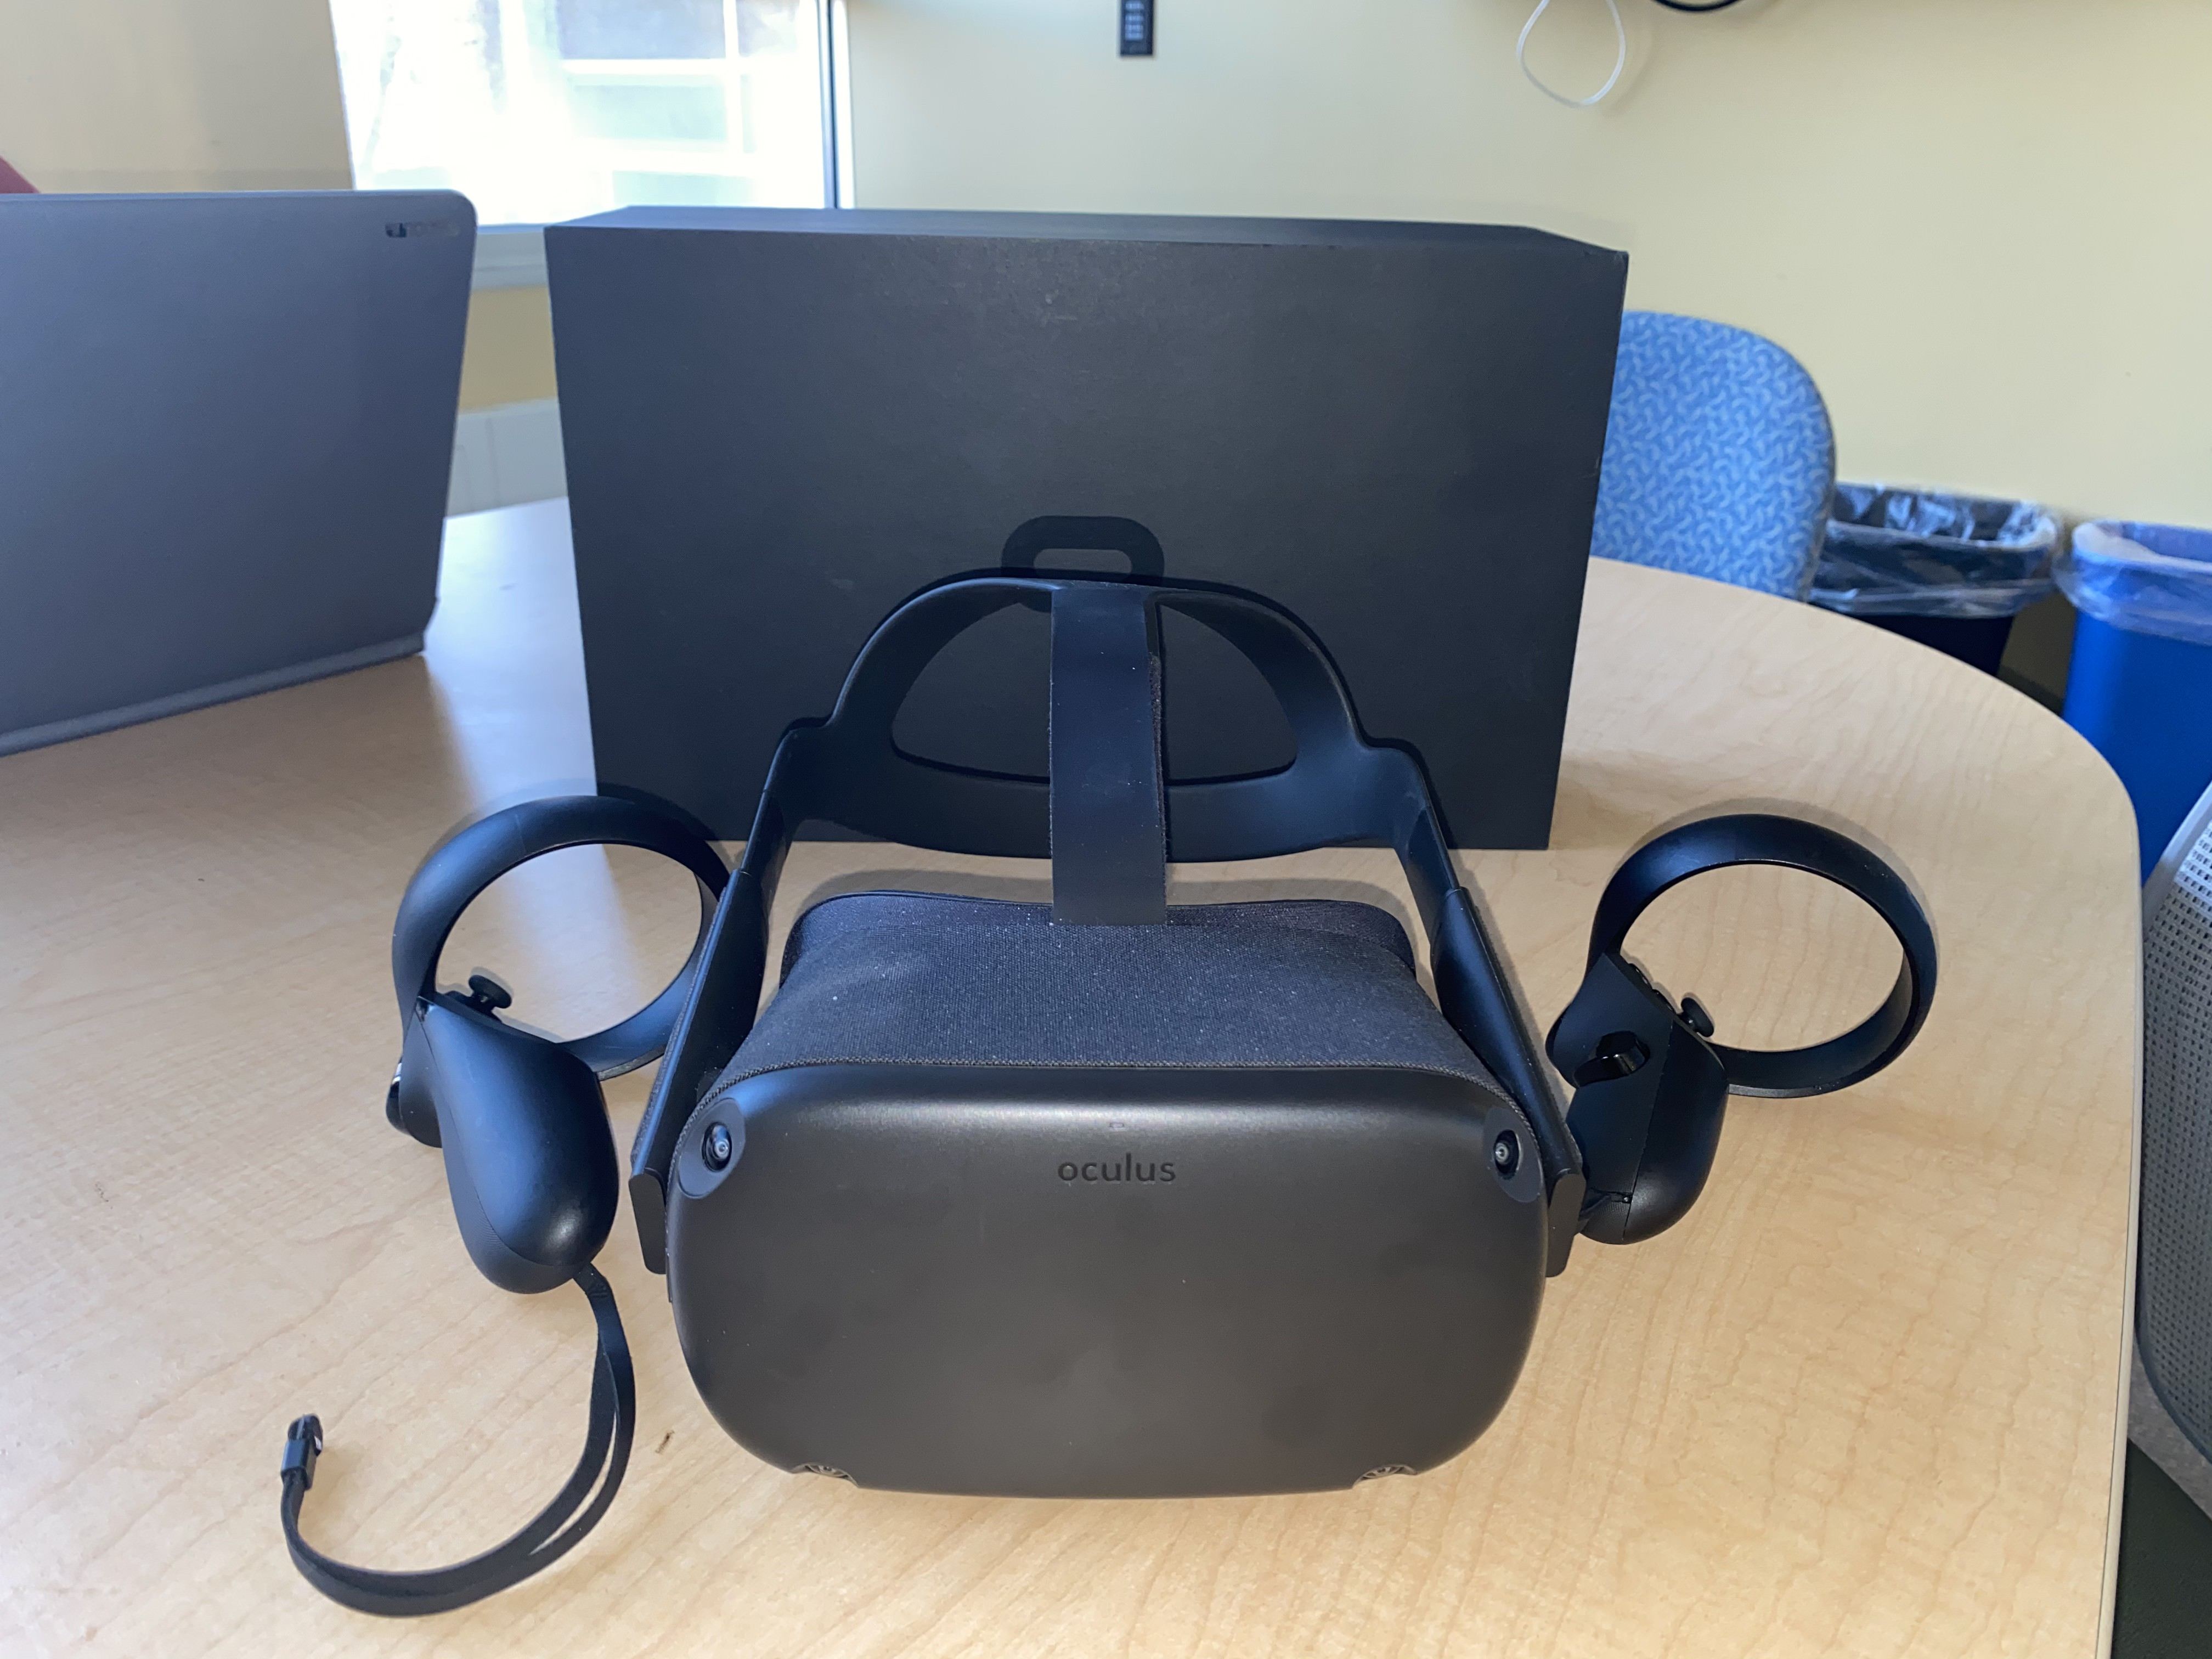
\includegraphics[scale=0.05]{figures/Oculus.jpg}
    \caption{Oculus Quest}
    \label{fig:my_label0}
\end{figure}

\subsection{Procedure}
To keep things consistent, all participants received the same instructions to eliminate any random variables and inconsistencies between the subjects. The participants also received two sets of instructions for the outside experiment and for the VR experiment. For the outdoor experiment participants were asked to use their fitness tracking wristbands to monitor their heart rate while they play the game. We chose fitness tracking wristbands because some of the participants did not feel confident in measuring their own heart rate, and wristband monitors only have around a 3-4\% error rate\cite{sarah_dinkel_john_m_noble_2016}. Only one person didn't have their own and borrowed one for the experiment. The users then were asked to play our version dodgeball where balls are thrown from various locations and at different speeds for five minutes and then answer questions. Afterwards participant’s heart rates were recorded and they have a rating based on how satisfied the activity was for them.  

The VR experiment had more instructions for the participants but with most of them already being familiar with the Oculus Quest it made instructions a lot more simple to explain to the participants. Prior to them starting the experiment the VR was set up and loaded with the game only requiring the participants to press start. They also used the same fitness trackers to monitor their heart rates from the outdoor experiments. Participants were instructed to hold the game controllers parallel to their body and move their entire body in order to dodge the incoming balls. After the game players heart rates were recorded and were also asked to rate their experience with the VR simulation. 


\setlength{\arrayrulewidth}{1mm}
\setlength{\tabcolsep}{8pt}
\renewcommand{\arraystretch}{1.25}
{\rowcolors{3}{gray!80}{white!70}
\begin{table}
\begin{tabularx}{0.45\textwidth}{ 
  | >{\centering\arraybackslash}X 
  | >{\centering\arraybackslash}X 
  | >{\centering\arraybackslash}X | }
\hline
Participant & Gender & Age \\
\hline
Participant 1 & male & 52 \\
\hline
Participant 2 & male & 22 \\
\hline
Participant 3 & female & 54 \\
\hline
Participant 4 & female & 30 \\
\hline
Participant 5 & male & 37 \\
\hline
Participant 6 & female & 22 \\
\hline
\end{tabularx}
\caption{Information about the participants}
\label{tab:my_label1}
\end{table}
}

We used a total of 6 different people listed on table 1 to conduct this experiment and all participants received the same instructions and demonstrations to keep things consistent among all the tests. We also made sure to ask all the participants for their heart rate at the same time after their experiment to avoid it going down from resting.  

\subsection{Task}
The task for this experiment is to test the enjoyment and likelihood of performing in a dodgeball type setting (reality and virtual reality) to see if using virtual reality is a liable option to introduce exercise to more people. This task will require the participants to complete a session of dodgeball outdoors, where the participants have to dodge balls that will come to them at various speeds and locations. This task will be repeated but in a virtual environment using an Oculus Quest. During these tasks, we will assess the intensity of the workout as well as the enjoyment and the likelihood of the participants wanting to repeat this exercise. There is a range of variables that will be measured and recorded in order to more accurately come to a valid conclusion that takes in the independent, dependent, random and controlled variables into consideration.

\begin{figure}
    \centering
    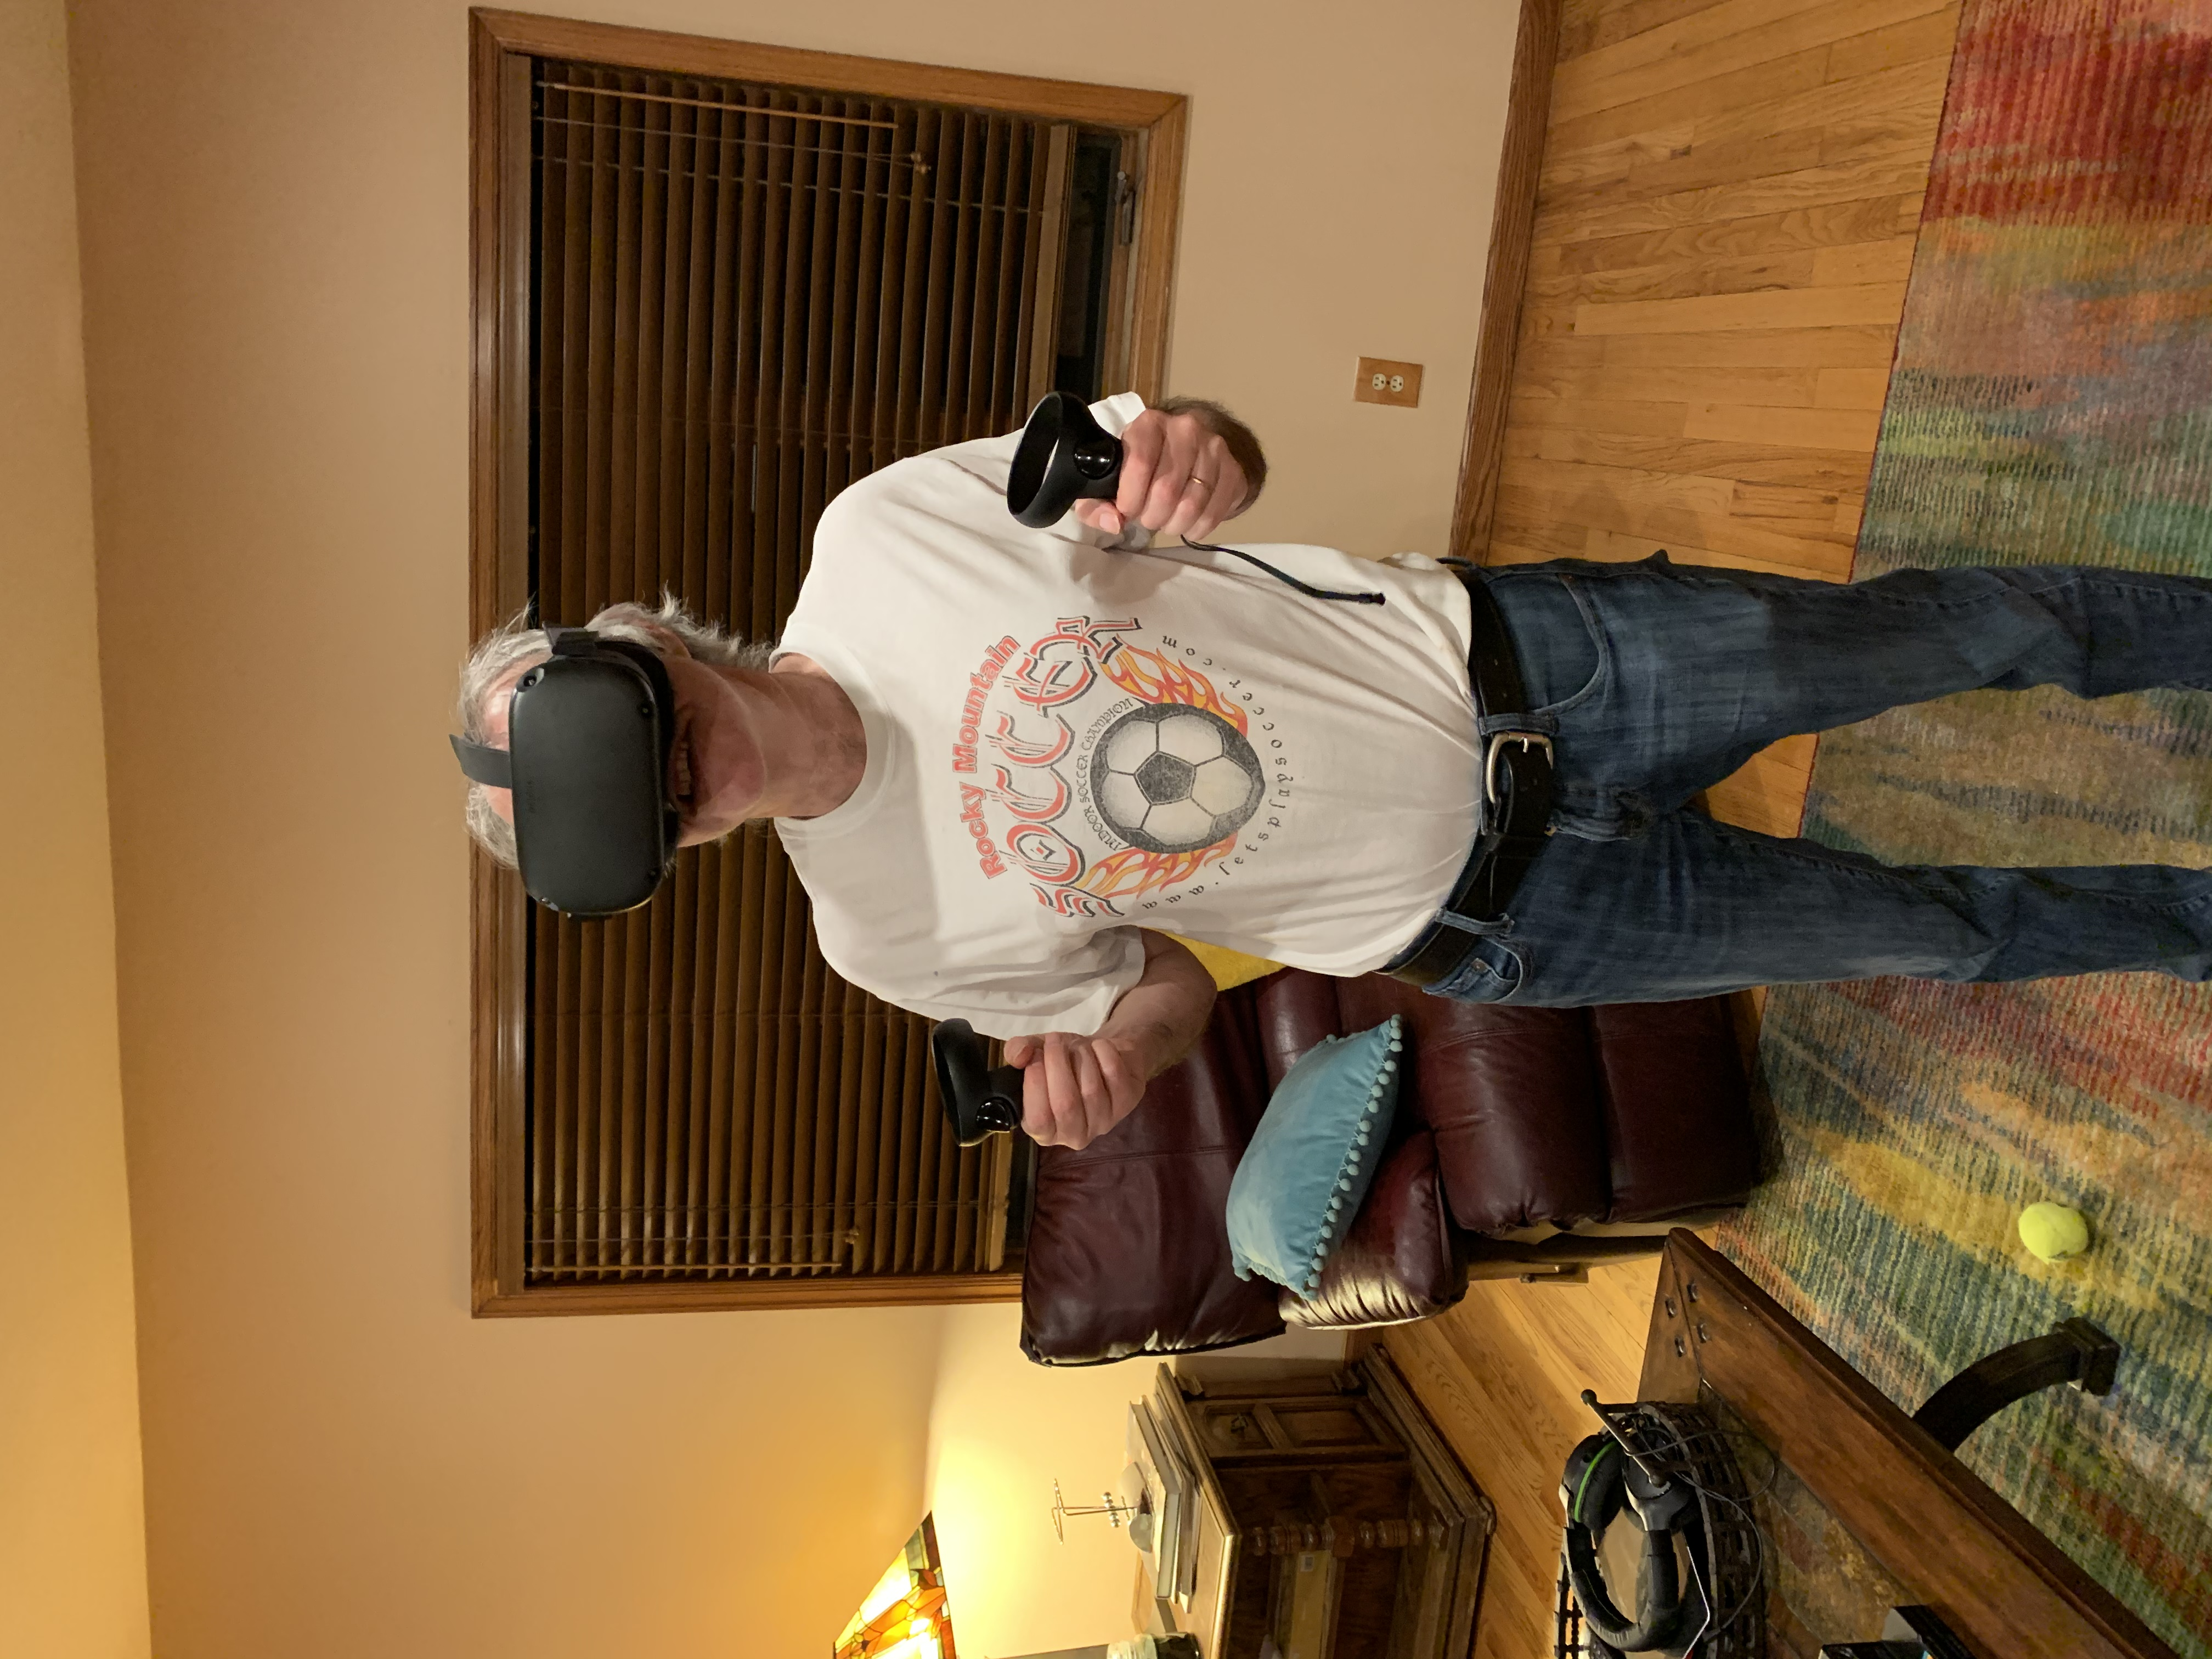
\includegraphics[scale=0.04, angle=270]{figures/Participant1.jpeg}
    \caption{Picture of participant 1 performing the experiment}
    \label{fig:my_label2}
\end{figure}

\begin{figure}
    \centering
    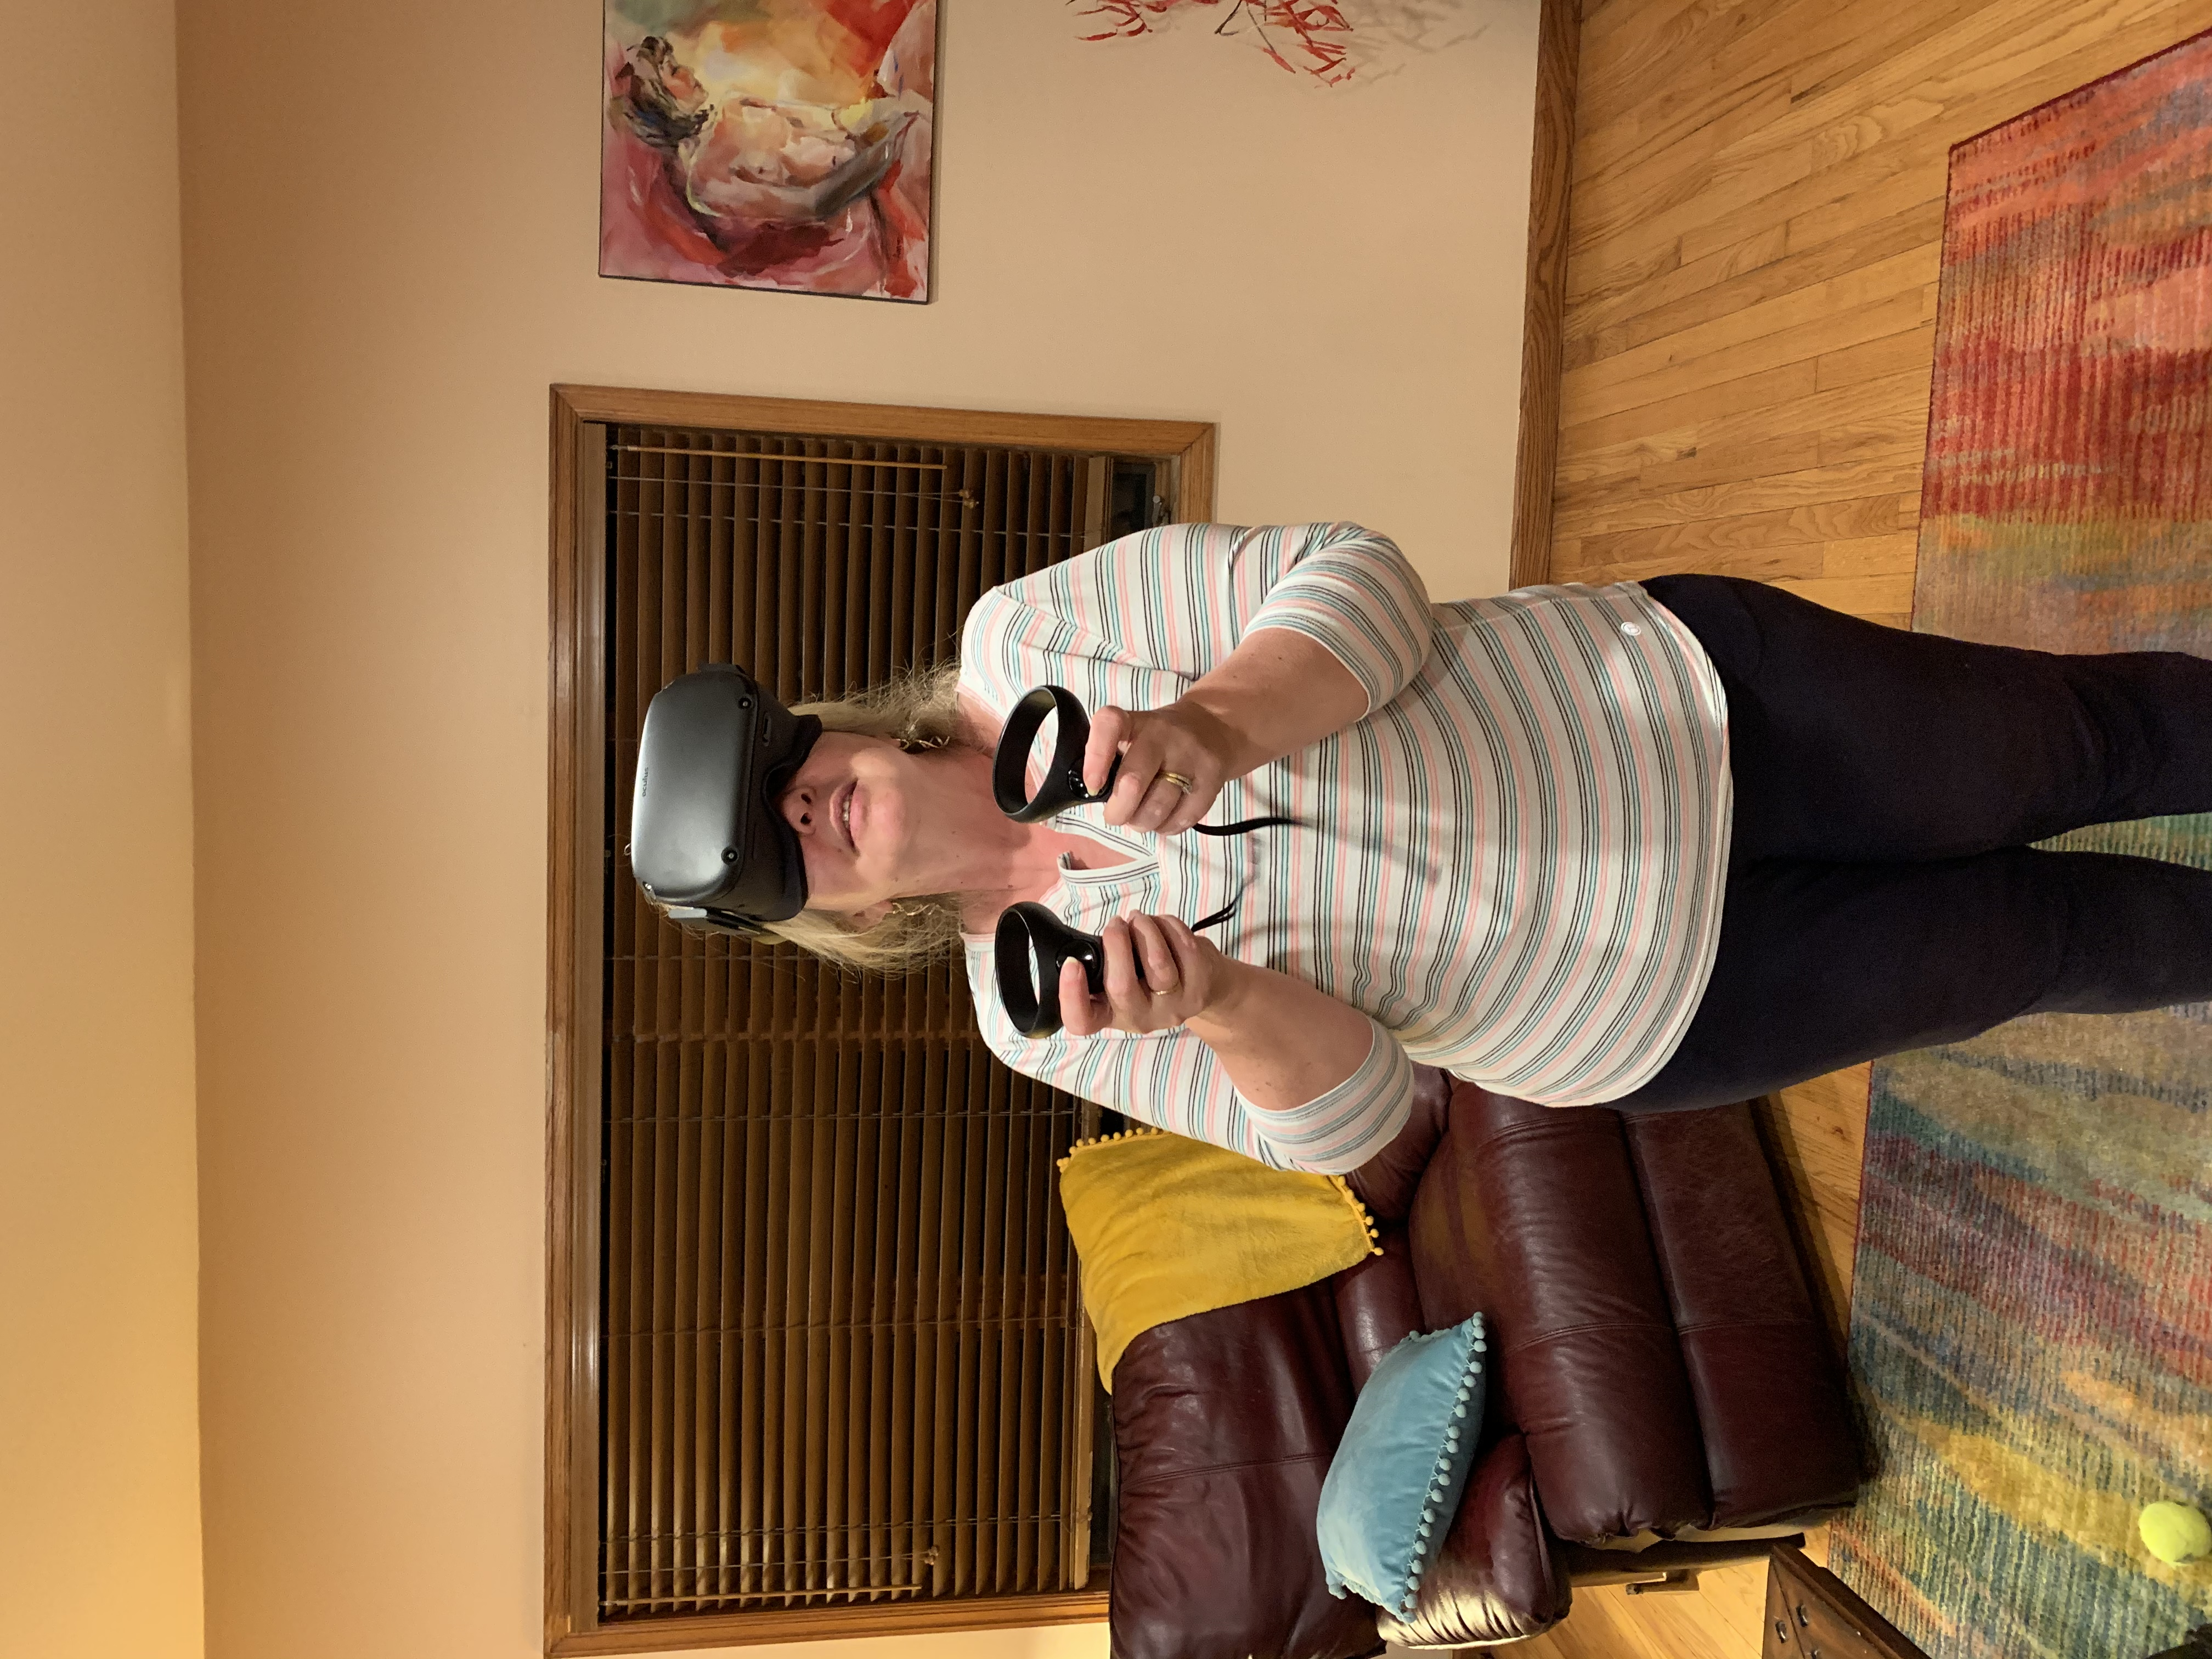
\includegraphics[scale=0.04, angle=270]{figures/Participant2.jpeg}
    \caption{Picture of participant 3 performing the experiment}
    \label{fig:my_label3}
\end{figure}

\subsection{Variables}
In this experiment, there are a lot of variables to take into account. However, due to the COVID-19 pandemic we have limited our variables. The independent variables are: setting (VR vs Real Life), Activity level of the Participants (sedentary, light, moderate, very active), and age. The dependent variables are: Heart rate, and user satisfaction (very dissatisfied, dissatisfied, neutral, satisfied, very satisfied). The random variables are: Temperature when experiment was performed, and the speed of which the ball travels. The control variables are: the VR headset used, the instructions we want the participants to follow, and the athleticism of the participant.

\section{Results and Discussion}
% Outdoor Setting
\setlength{\arrayrulewidth}{1mm}
\setlength{\tabcolsep}{8pt}
\renewcommand{\arraystretch}{1.25}
{\rowcolors{3}{gray!80}{white!70}
\begin{table}
\begin{tabularx}{0.45\textwidth}{ 
  | >{\centering\arraybackslash}X 
  | >{\centering\arraybackslash}X 
  | >{\centering\arraybackslash}X | }
\hline
Participant & Setting & Heart Rate(BPM) \\
\hline
1 & Outdoor & 102 \\
\hline
2 & Outdoor & 90 \\
\hline
3 & Outdoor & 127 \\
\hline
4 & Outdoor & 112 \\
\hline
5 & Outdoor & 120 \\
\hline
6 & Outdoor & 136 \\
\hline
\end{tabularx}
\caption{Table of Heart rate of participant after outdoor setting }
\label{tab:my_label4}
\end{table}
}

% Indoor Setting
\setlength{\arrayrulewidth}{1mm}
\setlength{\tabcolsep}{8pt}
\renewcommand{\arraystretch}{1.25}
{\rowcolors{3}{gray!80}{white!70}
\begin{table}
\begin{tabularx}{0.45\textwidth}{ 
  | >{\centering\arraybackslash}X 
  | >{\centering\arraybackslash}X 
  | >{\centering\arraybackslash}X | }
\hline
Participant & Setting & Heart Rate(BPM) \\
\hline
1 & Indoor & 73 \\
\hline
2 & Indoor & 71 \\
\hline
3 & Indoor & 85 \\
\hline
4 & Indoor & 79 \\
\hline
5 & Indoor & 81 \\
\hline
6 & Indoor & 90 \\
\hline
\end{tabularx}
\caption{Table of Heart rate of participant after indoor setting}
\label{tab:my_label5}
\end{table}
}

% Level of satisfaction after outdoor setting
\setlength{\arrayrulewidth}{1mm}
\setlength{\tabcolsep}{8pt}
\renewcommand{\arraystretch}{1.25}
{\rowcolors{3}{gray!80}{white!70}
\begin{table}
\begin{tabularx}{0.45\textwidth}{ 
  | >{\centering\arraybackslash}X 
  | >{\centering\arraybackslash}X 
  | >{\centering\arraybackslash}X | }
\hline
Participant & Activity Level  & Satisfaction Level \\
\hline
1 & Moderate & Satisfied \\
\hline
2 & Very Active & Very Satisfied \\
\hline
3 & Sedentary & Neutral \\
\hline
4 & Moderate & Dissatisfied \\
\hline
5 & Light & Dissatisfied \\
\hline
6 & Light & Neutral \\
\hline
\end{tabularx}
\caption{Table of Activity level and Satisfaction level of participants after outdoor setting}
\label{tab:my_label6}
\end{table}
}

% Level of satisfaction after indoor setting
\setlength{\arrayrulewidth}{1mm}
\setlength{\tabcolsep}{18pt}
\renewcommand{\arraystretch}{1.25}
{\rowcolors{3}{gray!80}{white!70}
\begin{table}
\begin{tabularx}{0.45\textwidth}{ 
  | >{\centering\arraybackslash}X 
  | >{\centering\arraybackslash}X 
  | >{\centering\arraybackslash}X | }
\hline
Participant & Activity Level  & Satisfaction Level \\
\hline
1 & Moderate & Satisfied \\
\hline
2 & Very Active & Dissatisfied \\
\hline
3 & Sedentary & Very Satisfied \\
\hline
4 & Moderate & Satisfied \\
\hline
5 & Light & Satisfied \\
\hline
6 & Light & Very Satisfied \\
\hline
\end{tabularx}
\caption{Table of Activity level and Satisfaction level of participants after indoor setting}
\label{tab:my_label7}
\end{table}
}

\begin{figure}
    \centering
    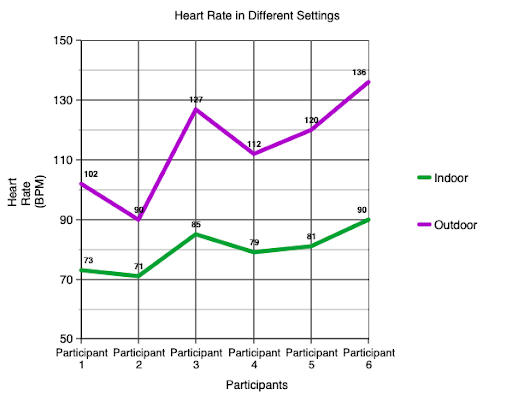
\includegraphics[scale=0.45]{figures/Heart_rate.png}
    \caption{Heart rate of participants in different settings}
    \label{fig:my_label8}
\end{figure}

\begin{figure}
    \centering
    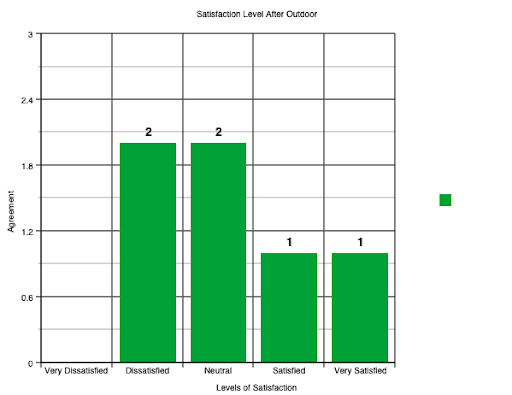
\includegraphics[scale=0.4]{figures/Outdoor_setting.png}
    \caption{Survey after outdoor setting}
    \label{fig:my_label9}
\end{figure}

\begin{figure}
    \centering
    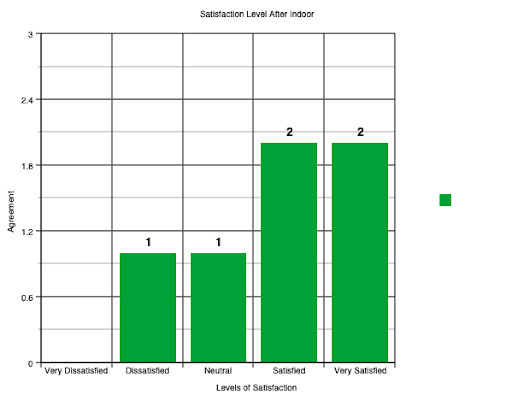
\includegraphics[scale=0.4]{figures/Indoor_setting.png}
    \caption{Survey after indoor setting}
    \label{fig:my_label10}
\end{figure}

% ANOVA
\setlength{\arrayrulewidth}{1mm}
\setlength{\tabcolsep}{8pt}
\renewcommand{\arraystretch}{1.25}
{\rowcolors{4}{gray!80}{white!70}
\begin{table}
\begin{tabularx}{0.45\textwidth}{ 
  | >{\centering\arraybackslash}X 
  | >{\centering\arraybackslash}X 
  | >{\centering\arraybackslash}X
  | >{\centering\arraybackslash}X |}
\hline
 & 1 & 2 & Total \\
\hline
N & 5 & 5 & 10 \\
\hline
$$\sum_{}^{} X$$ & 6 & 6 & 12 \\
\hline
Mean & 1.2 & 1.2 & 1.2 \\
\hline
$$\sum_{}^{} X^2$$ & 10 & 10 & 20 \\
\hline
Std. Dev & 0.8367 & 0.8367 & 0.7888 \\
\hline
\end{tabularx}
\caption{ANOVA test results }
\label{tab:my_label12}
\end{table}
}

After conducting the experiment and looking at figures 5 and 6, it seems like there was a change in the enjoyment of the participants, and the participants enjoyed the indoor setting of our game versus the outdoor setting. Also, looking at figure 4, the average heart rate for the indoor settings was lower than the outdoor setting, meaning people who do not exercise a lot would have a greater chance of enjoying it as it is not as physically exhausting \cite{teixeira_2012}.  However, this is not a significant result. After running the one-way ANOVA, it shows after having the participants play in both settings, the difference was not significant ( t = 0.0, df = 10, p > .05 ). Since the p-value > $\alpha$,  H0 is accepted. The averages of both groups are considered to be equal. However, the difference between the averages of all groups is not big enough to be statistically significant. Due to the pandemic we had to shrink the participant pool, which drastically changed the effectiveness, and the results of this experiment. The smaller the pool, the larger the deviations can be \cite{simmons_2019}. Even though at a glance it looked significant it is because the deviations were big (around 1.87). Thus, we cannot conclude that our indoor game of dodgeball is just as enjoyable as the outdoor counterpart. 

\section{Conclusion}
We created a game that attempted to introduce users of various ages and physical activity lifestyles to dodgeball. This was attempted using VR, which allowed the player to move and act as if they were playing the real game. We tested how players would react to the VR and real version of the game while recording data that we later used and discussed in the Results section of our report. Unfortunately, given the global pandemic our sample size was too small and results were inconclusive. We then evaluated how we could improve the game to make it more enjoyable while also trying to get as close as possible to the physical challenge of the real game.

After performing these experiments, we found many interesting takes on performing exercise using Virtual Reality. Although we found that only about half of the participants that we tested were satisfied with the VR activity over the outdoor game, most of them enjoyed it as a fun way to just play a game and compete against each other to see who can perform the best. This may not bring as much physical exertion as outdoor dodgeball but it could prompt users to play it more often which could then lead to more total exercise being done in the long run. This would require more testing and another future experiment to test if users are more likely to keep playing it indoors especially with the current pandemic that is happening. 

There are plenty of features we would implement if there was more time allocated to develop this project. Some of these features include allowing the user to choose from an array of different levels of difficulty so that the experience is personalized to them and their fitness level. Implementing this feature would not be difficult since our logic was designed in such a way we could change the speed at which the dodgeballs are thrown by changing a single variable, spawning a different amount of dodgeballs works similarly. The more challenging part of levels of difficulties would be the unity side of things since implementing a working user interface is something we struggled with. Another feature that could significantly help with immersion would be the addition of realistic physics which was not our focus this semester, realistic physics would match the user’s real life experiences and provide a better overall experience. Lastly, most users tried to catch the dodgeballs out of instinct which unfortunately was not supported.   

\balance{}

\balance{}

% REFERENCES FORMAT
% References must be the same font size as other body text.
\bibliographystyle{SIGCHI-Reference-Format}
\bibliography{sample}

\end{document}

%%% Local Variables:
%%% mode: latex
%%% TeX-master: t
%%% End:
